\section{Auswertung}
\label{sec:Auswertung}

\subsection{Das Spektrum der $^{137}$Cs-Quelle}
In Abbildung \ref{fig:tfig1} ist das Spektrum der verwendeten $^{137}$Cs-Quelle zu sehen.
Die auf der $x$-Achse aufgetragenen Kanäle sind ein Maß für die Energie der gemessenen Photonen.

\begin{figure}
\centering
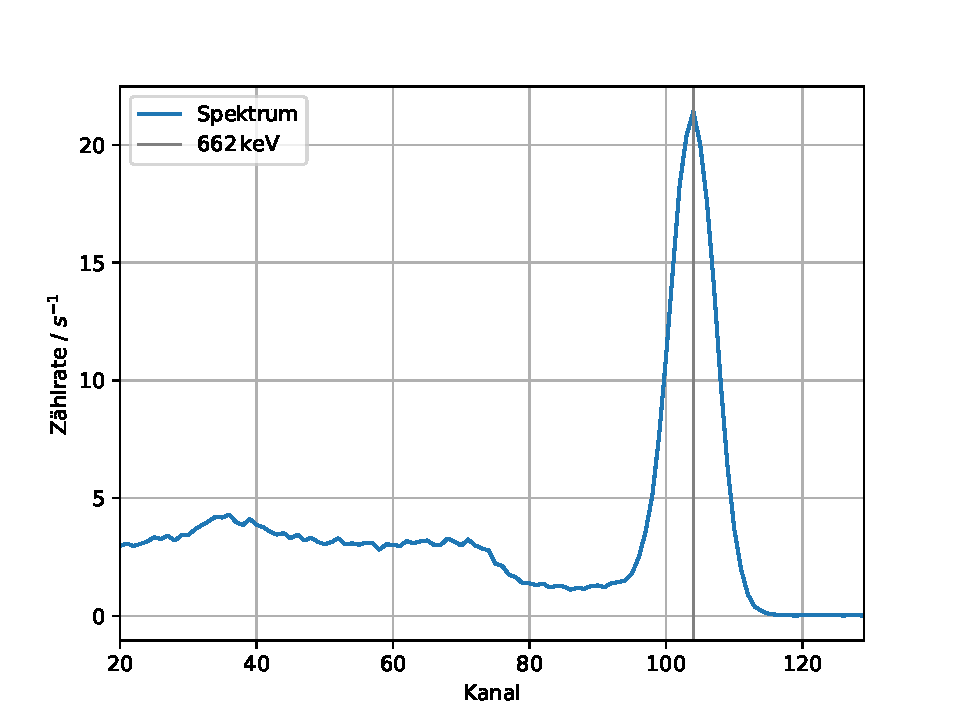
\includegraphics[width=0.8\textwidth]{figures/Spektrum}
\caption{Das Spektrum der $^{137}$Cs-Quelle. Aufgetragen sind die Zählraten der einzelnen Kanäle, welche ein Maß für die Energie der detektierten Photonen sind.
Deutlich zu erkennen ist das Compton-Kontinuum und der Photopeak bei einer Energie von $E_\gamma = \SI{662}{\keV}$.}
\label{fig:tfig1}
\end{figure}

Der Compton-Effekt ist die Streuung eines Photons an einem Elektron des Szintillatormaterials.
Durch diesen erfahren die Photonen je nach Streuwinkel einen unterschiedlich starken Energieverlust, sodass sich ein kontinuierliches Compton-Kontinuum ergibt.
Dieses reicht etwa bis zu dem Kanal $75$ und endet dort abrupt mit der Compton-Kante, welche den maximalen Energieverlust bei einem Streuwinkel von $180°$ darstellt.

Bei dem Photoneffekt gibt das Photon seine gesamte Energie auf ein Hüllenelektron ab.
Die Lage des Photopeaks repräsentiert also die Gesamtenergie der eingestrahlten Photonen.
Für die hier verwendete $^{137}$Cs-Quelle liegt das Maximum des Photopeaks bei dem Kanal $104$, was einer Energie von $E_\gamma = \SI{662}{\keV}$ entspricht.

\subsection{Bestimmung der Absorptionskoeffizienten}
In den Tabellen \ref{tab:ttab1} bis \ref{tab:ttab4} befinden sich die gemessenen Counts für die verschiedenen Würfel, sowie die Messdauer.
Hierbei handelt es sich bei dem Würfel 1 um den leeren Würfen, an welchem die Größe $I_0$ gemessen wird.
Würfel 2 und 3 sind aus je einem homogenen Material, während Würfel 5 aus diesen beiden Materialien zusammengesetzt ist.

Die Zählrate ergibt sich durch
\begin{equation}
    N = \frac{C}{t}\, .
\end{equation}
Wobei sich der Fehler mittels Gauß'scher Fehlerfortpflanzung
\begin{equation}
    \sigma_f = \sqrt{\sum_i \left(\frac{\partial f}{\partial x_i}\sigma_{x_i}\right)^2}
\end{equation}
zu
\begin{equation}
    \sigma_N = \frac{\sigma_C}{t}
\end{equation}
ergibt.

\subsubsection*{Würfel 1}
Bei dem leeren Würfel wurden die drei Projektionen $I_2$, $I_3$ und $I_5$ gemessen.
Die Zählraten dieser Messungen dienen im Folgenden als $I_0$, sodass der Einfluss der Aluminiumhülle des Würfels berücksichtigt ist.

\begin{table} 
\caption{Messwerte des hohlen Würfels 1. Gemessen wurden die Projektionen $I_2,\, I_3,\, \text{und}\, I_5$}
\label{tab:ttab1}
\centering
\begin{tabular}{s | S[] S[] r}
\toprule
    {Projektion} & {$C$} & {$t/\si{\s}$} & {$I_0/\symup{s^{-1}}$} \\
    \midrule
    I_2 & 22860\pm 231 & 200,08 &  114 \pm 1 \\
    I_3 & 21185\pm 251 & 200,16 &  106 \pm 1 \\
    I_5 & 32699\pm 217 & 200,52 &  163 \pm 1\\
\end{tabular}
\end{table}

\subsubsection*{Würfel 2}
Da im Falle der homogenen Würfel keine Korrelation vorliegt, wird der Absorptionskoeffizient durch Umformung der Gleichung \eqref{eq:linearKoeff} zu
\begin{equation}
    \mu_i = \frac{I_i}{d_i} \qquad \text{mit} \qquad I_i = \ln\left(\frac{I_0}{N_j}\right)
\end{equation}
berechnet.
Hierbei muss nur beachtet werden, dass die Strecke $d_i$, die die Strahlung in dem Material zurücklegt, je nach Projektion variiert.
Die Absorptionskoeffizienten, welche sich für den Würfel 2 ergeben, sind in Tabelle \ref{tab:ttab2} aufgeführt.
Die zugehörigen Fehler werden mittels Gauß'scher Fehlerfortpflanzung
\begin{equation}
    \sigma_\mu = \frac{1}{d_i}\sqrt{\left(\frac{\sigma_{I_i}}{I_i}\right)^2+\left(\frac{\sigma_{I_0}}{I_0}\right)}
\end{equation}
bestimmt.
Somit ergibt sich im Mittel ein Absorptionskoeffizient von
\begin{equation}
    \mu_{\text{W}_2} = \SI{0,613\pm 0,005}{\per\cm}\, .
\end{equation}
Bei einer Dichte von $\rho_\text{Fe} = \SI{7,874}{\g\per\cm\cubed}$ \cite{rho} beträgt der Absorptionskoeffizient von Eisen $\mu_\text{Fe,lit} = \SI{0,607}{\per\cm}$ \cite{mu}, von welchem der des zweiten Würfels um $1\%$ abweicht.
Somit wird angenommen, dass es sich bei dem Material des Würfels 2 um Eisen handelt.

\begin{table} 
\caption{Messwerte des homogenen Würfels 2. Gemessen wurden die Projektionen $I_2,\, I_3,\, \text{und}\, I_5$}
\label{tab:ttab2}
\centering
\begin{tabular}{s | S[] S[] c c c}
\toprule
    {Projektion} & {$C$} & {$t/\si{\s}$} & {$N/\symup{s^{-1}}$} & {$d/\si{\cm}$} & {$\mu/\symup{cm^{-1}}$}\\
    \midrule
    I_2 & 2811\pm 78 & 201,18 & 14,0\pm 0,4 & $3\sqrt{2}$ & 0,495\pm 0,007 \\
    I_3 & 2828\pm 94 & 200,46 & 14,1\pm 0,5 & $2\sqrt{2}$ & 0,712\pm 0,012 \\
    I_5 & 5218\pm 98 & 211,9  & 24,6\pm 0,5 & $3$         & 0,630\pm 0,007 \\
\end{tabular}
\end{table}

\subsubsection*{Würfel 3}
Für den anderen homogenen Würfel 3 wird analog vorgegangen. 
Die entsprechenden Werte sind in Tabelle \ref{tab:ttab3} zu sehen.
Hier ergibt sich ein mittlerer Absorptionskoeffizient von
\begin{equation}
    \mu_{\text{W}_3} = \SI{0,089\pm 0,003}{\per\cm}\, .
\end{equation}
Folglich wird angenommen, dass es sich bei dem Material des Würfels 3 um Delrin handelt, welches bei einer Dichte von $\rho_\text{D} = \SI{1,41}{\g\per\cm\cubed}$ \cite{rho} einen Absorptionskoeffizienten von $\mu_\text{D,lit} = \SI{0,12}{\per\cm}$ \cite{mu} aufweist.


\begin{table} 
\caption{Messwerte des homogenen Würfels 3. Gemessen wurden die Projektionen $I_2,\, I_3,\, \text{und}\, I_5$}
\label{tab:ttab3}
\centering
\begin{tabular}{s | S[] S[] S c c}
\toprule
    {Projektion} & {$C$} & {$t/\si{\s}$} & {$N/\symup{s^{-1}}$}& {$d/\si{\cm}$} & {$\mu/\symup{cm^{-1}}$} \\
    \midrule
    I_2 & 14677\pm 204 & 200,24 & 73\pm  1 & $3\sqrt{2}$ &  0,105\pm 0,004\\
    I_3 & 18800\pm 198 & 200,54 & 94\pm  1 & $2\sqrt{2}$ &  0,043\pm 0,006\\
    I_5 & 23950\pm 189 & 209,24 & 114\pm 1 & $3$         &  0,118\pm 0,003\\
\end{tabular}
\end{table}

\subsubsection*{Würfel 5}
Die Zählraten der Projektionen $I_1$ bis $I_{12}$ des inhomogenen Würfels 5 sind in Tabelle \ref{tab:ttab4} aufgeführt.
\begin{table} 
    \caption{Messwerte des unbekannten Würfels 5. Gemessen wurden die Projektionen $I_1$ bis $I_{12}$. Die Messdauer beträgt bei allen Messungen $t=\SI{300}{\s}$.}
    \label{tab:ttab4}
    \centering
    \begin{tabular}{s | S[] c}
    \toprule
        {Projektion} & {$C$} & {$N/\symup{s^{-1}}$} \\
        \midrule
        I_1    & 15969\pm 183 & 53,23\pm 0,6\\
        I_2    & 10120\pm 169 & 33,73\pm 0,6\\
        I_3    & 9002\pm 189  & 30,00\pm 0,6\\
        I_4    & 5962\pm 131  & 19,87\pm 0,4\\
        I_5    & 13244\pm 183 & 44,15\pm 0,6\\
        I_6    & 14699\pm 202 & 49,00\pm 0,7\\
        I_7    & 11592\pm 130 & 38,64\pm 0,4\\
        I_8    & 8668\pm 113  & 28,89\pm 0,4\\
        I_9    & 24658\pm 186 & 82,19\pm 0,6\\
        I_{10} & 7484\pm 119  & 24,95\pm 0,4\\
        I_{11} & 17332\pm 204 & 57,77\pm 0,7\\
        I_{12} & 18130\pm 190 & 60,43\pm 0,6\\
    \end{tabular}
    \end{table}

Dieser Würfel ist aus den Materialien der Würfel 2 und 3 zusammengesetzt.
Die einzelnen Elementarwürfel besitzen somit unterschiedliche Absorptionskoeffizienten, welche das Gleichungssystem \eqref{eq:LGS_mu} mit 
\begin{equation}
    A = \SI{1}{\cm}\cdot 
    \begin{pmatrix}
        0 & 0 & 0 & 0 & 0 & \sqrt{2} & 0 & \sqrt{2} & 0 \\
        0 & 0 & \sqrt{2} & 0 & \sqrt{2} & 0 & \sqrt{2} & 0 & 0 \\
        0 & \sqrt{2} & 0 & \sqrt{2} & 0 & 0 & 0 & 0 & 0 \\
        0 & 0 & 0 & 0 & 0 & 0 & 1 & 1 & 1 \\
        0 & 0 & 0 & 1 & 1 & 1 & 0 & 0 & 0 \\
        1 & 1 & 1 & 0 & 0 & 0 & 0 & 0 & 0 \\
        0 & 0 & 0 & \sqrt{2} & 0 & 0 & 0  & \sqrt{2} & 0 \\
        \sqrt{2} & 0 & 0 & 0 & \sqrt{2} & 0 & 0 & 0 & \sqrt{2} \\
        0 & \sqrt{2} & 0 & 0 & 0  & \sqrt{2} & 0 & 0 & 0\\
        1 & 0 & 0 & 1 & 0 & 0 & 1 & 0 & 0 \\
        0 & 1 & 0 & 0 & 1 & 0 & 0 & 1 & 0 \\
        0 & 0 & 1 & 0 & 0 & 1 & 0 & 0 & 1 \\
      \end{pmatrix}
\end{equation}
erfüllen.
Aufgrund der Korrelation zwischen den Absorptionskoeffizienten lassen sich die Fehler nicht mehr durch die Gauß'sche Fehlerfortpflanzung berechnen, sondern entsprechen der Wurzel der Diagonalelemente der Kovarianzmatrix \eqref{eq:kov}
\begin{equation}
    \sigma_{\mu_i} = \sqrt{V[\vec{\mu}]_{ii}} \, .
\end{equation}
Die berechneten Absorptionskoeffizienten der Elementarwürfel $1$ bis $9$ sind in Tabelle \ref{tab:ttab5} aufgeführt.
Um die Elementarwürfel jeweils einem Material zuordnen zu können, sind zusätzlich die absoluten Abweichungen zu den gemessenen Absorptionskoeffizienten sowie zu den Literaturwerten angegeben.
Den Würfeln wird dann das Element zugeordnet bei welchem die geringste Abweichung vorliegt.
Die Zusammensetzung des Würfels ist in Abbildung \ref{fig:tfig2} dargestellt.

\begin{table} 
\caption{Absorptionskoeffizienten der Elementarwürfel des Würfels 5 und die jeweiligen Abweichungen zu den experimentellen Absorptionskoeffizienten und Literaturwerten.
Die fett gedruckten Abweichungen sind jeweils die betragsmäßig kleinsten, sodass dem Elementarwürfel dieser Stoff zugeordnet wird, wie in Abbildung \ref{fig:tfig2} dargestellt ist.}
\label{tab:ttab5}
\centering
\begin{tabular}{c | c c c c c c}
\toprule
    {} & {$\mu/\symup{cm^{-1}}$} & {$|\Delta\mu_\text{Fe,lit}|$} & {$|\Delta\mu_\text{Fe,exp}|$} & {$|\Delta\mu_\text{D,lit}|$} & {|$\Delta\mu_\text{D,exp}|$}  \\
    \midrule
    $\mu_1$ & 0,425\pm 0,011 & \textbf{0,182} & 0,188 & 0,305 & 0,336 \\
    $\mu_2$ & 0,312\pm 0,008 & 0,295 & 0,301 & \textbf{0,192} & 0,223 \\
    $\mu_3$ & 0,162\pm 0,010 & 0,445 & 0,451 & \textbf{0,042} & 0,073 \\
    $\mu_4$ & 0,596\pm 0,009 & \textbf{0,011} & 0,017 & 0,476 & 0,507 \\
    $\mu_5$ & 0,096\pm 0,008 & 0,511 & 0,517 & 0,024 & \textbf{0,007} \\
    $\mu_6$ & 0,127\pm 0,008 & 0,480 & 0,486 & \textbf{0,007} & 0,038 \\
    $\mu_7$ & 0,789\pm 0,012 & 0,182 & \textbf{0,176} & 0,669 & 0,700 \\
    $\mu_8$ & 0,377\pm 0,008 & \textbf{0,230} & 0,236 & 0,257 & 0,288 \\
    $\mu_9$ & 0,636\pm 0,011 & 0,029 & \textbf{0,023} & 0,516 & 0,547 \\
    
\end{tabular}
\end{table}

\begin{figure}
\centering
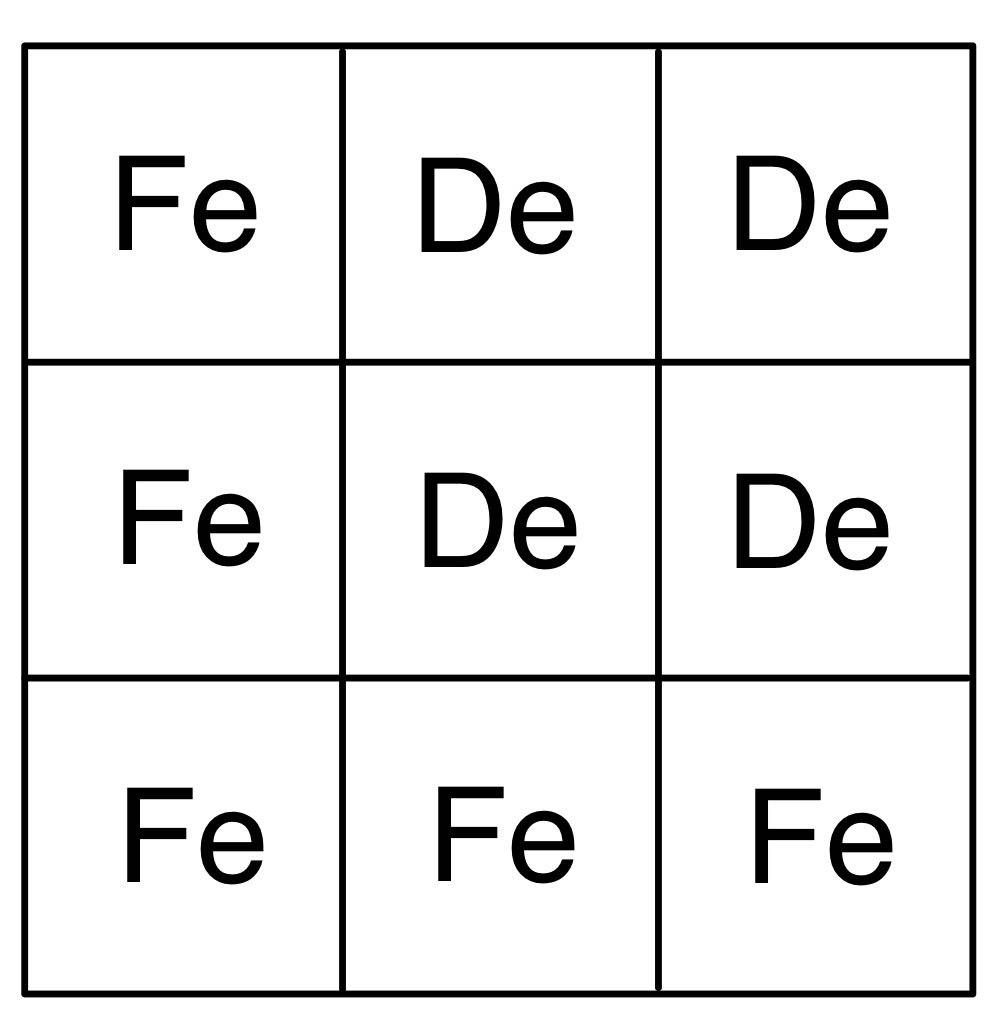
\includegraphics[width=0.3\textwidth]{figures/W5}
\caption{Experimentell bestimmte Zusammensetzung des Würfel 5.}
\label{fig:tfig2}
\end{figure}